% !TEX program = lualatex
\documentclass[border=6pt]{standalone}
% ---------------------------------------------------------------------------
% tikzpreamble.tex -- shared by main.tex and by every standalone in tikz/
% ---------------------------------------------------------------------------
\usepackage{amsmath}
\usepackage{amssymb}
\usepackage{tikz}
\usepackage{circuitikz}
\usetikzlibrary{arrows.meta,calc,positioning,decorations.pathmorphing,decorations.pathreplacing,
                decorations.markings,patterns,angles,quotes,fit,
                shapes.geometric,shapes.misc,backgrounds,intersections}

\ctikzset{bipoles/length=0.85cm}
\ctikzset{resistors/scale=0.85}
\ctikzset{capacitors/scale=0.9}

\tikzset{
  wire/.style      = {line width=0.7pt},
  dashedwire/.style= {line width=0.7pt, densely dashed},
  term/.style      = {circle, draw, line width=0.6pt, fill=white,
                      inner sep=0pt, minimum size=4.5pt},
  node dot/.style  = {circle, fill=black, inner sep=0pt, minimum size=4pt},
  boxlabel/.style  = {font=\sffamily\small},
  annot/.style     = {font=\small, align=left},
  phasor/.style    = {-{Stealth[length=3.2mm,width=2.2mm]}, line width=1.1pt},
  thinphasor/.style= {-{Stealth[length=2.6mm,width=1.8mm]}, line width=0.7pt},
  axis line/.style = {-{Stealth[length=2.6mm,width=1.8mm]}, line width=0.6pt},
  guide/.style     = {densely dashed, line width=0.4pt, gray},
}
\usepackage{siunitx}

\begin{document}
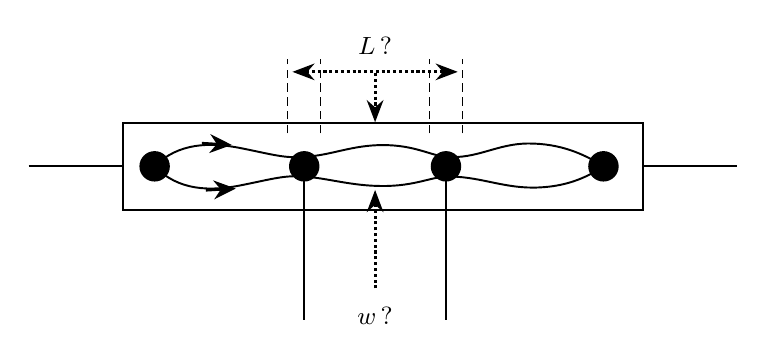
\begin{tikzpicture}[
    every node/.style={font=\small},
    bigdot/.style={circle, fill=black, inner sep=0pt, minimum size=11pt},
    dimline/.style={line width=1.1pt, densely dotted},
  ]

  % ---- sample strip and current leads ------------------------------------
  \draw[wire] (1.4,-0.55) rectangle (8.0,0.55);
  \draw[wire] (0.2,0) -- (1.4,0);
  \draw[wire] (8.0,0) -- (9.2,0);

  % ---- irregular current-flow lines --------------------------------------
  % They pinch at each contact dot and bulge out in between, so the effective
  % path length between the voltage contacts is ill-defined.
  \draw[wire]
      (1.8,0)  .. controls (2.10,0.30) and (2.50,0.31) .. (2.90,0.23)
               .. controls (3.30,0.15) and (3.45,0.10) .. (3.70,0.12)
               .. controls (4.05,0.14) and (4.30,0.27) .. (4.70,0.27)
               .. controls (5.10,0.27) and (5.30,0.14) .. (5.50,0.12)
               .. controls (5.90,0.09) and (6.15,0.29) .. (6.55,0.29)
               .. controls (6.95,0.29) and (7.25,0.16) .. (7.50,0);
  \draw[wire]
      (1.8,0)  .. controls (2.10,-0.31) and (2.50,-0.32) .. (2.90,-0.24)
               .. controls (3.30,-0.16) and (3.45,-0.11) .. (3.70,-0.13)
               .. controls (4.00,-0.15) and (4.30,-0.25) .. (4.70,-0.25)
               .. controls (5.10,-0.25) and (5.30,-0.14) .. (5.50,-0.13)
               .. controls (5.90,-0.12) and (6.20,-0.27) .. (6.60,-0.27)
               .. controls (7.00,-0.27) and (7.28,-0.15) .. (7.50,0);

  \draw[-{Stealth[length=2.8mm,width=2.4mm]},line width=0.9pt]
        (2.40,0.295) -- (2.78,0.272);
  \draw[-{Stealth[length=2.8mm,width=2.4mm]},line width=0.9pt]
        (2.45,-0.305) -- (2.83,-0.282);

  % ---- the four contacts, drawn large: their size is the whole problem ----
  \foreach \x in {1.8,3.7,5.5,7.5} { \node[bigdot] at (\x,0) {}; }

  % ---- voltage leads from the two inner contacts -------------------------
  \draw[wire] (3.7,0) -- (3.7,-1.95);
  \draw[wire] (5.5,0) -- (5.5,-1.95);

  % ---- L?  : a pair of extension lines straddles each contact dot --------
  \foreach \x in {3.49,3.91,5.29,5.71} { \draw[guide,black] (\x,0.42) -- (\x,1.36); }
  \draw[dimline,{Stealth[length=2.8mm]}-{Stealth[length=2.8mm]}] (3.55,1.20) -- (5.65,1.20);
  \node[anchor=south] at (4.6,1.30) {$L$\,?};
  \draw[dimline,-{Stealth[length=2.8mm]}] (4.6,1.18) -- (4.6,0.56);

  % ---- w?  : arrow pointing up into the strip ----------------------------
  \draw[dimline,-{Stealth[length=2.8mm]}] (4.6,-1.55) -- (4.6,-0.30);
  \node[anchor=north] at (4.6,-1.66) {$w$\,?};
\end{tikzpicture}
\end{document}
